\documentclass{article}
\usepackage[utf8]{inputenc}
\usepackage[italian]{babel}
\usepackage[margin=1.25in]{geometry}

\usepackage{amsfonts, amssymb}
\usepackage{amsmath, amsthm}
\usepackage[thicklines]{cancel}

\usepackage{graphicx}
\usepackage{hyperref}

\hypersetup{
colorlinks=true,
linkcolor=black,
filecolor=magenta,
urlcolor=blue,
}

\newtheorem*{thm}{Teorema}

\theoremstyle{definition}
\newtheorem*{dfn}{Definizione}
\newtheorem*{oss}{Osservazione}
\newtheorem*{dms}{Dimostrazione}
\newtheorem*{eg}{Esempio}
\newtheorem*{nb}{N.B}

\newcommand{\quoted}[1]{``#1''}
\newcommand{\angled}[1]{\langle #1 \rangle}
\newcommand{\numN}{\mathbb{N}}
\newcommand{\numZ}{\mathbb{Z}}
\newcommand{\numQ}{\mathbb{Q}}
\newcommand{\numR}{\mathbb{R}}

\newcommand{\gap}{\hspace{.4cm}}
\newcommand{\ggap}{\hspace{.6cm}}
\newcommand{\Gap}{\hspace{1cm}}
\newcommand{\GAP}{\hspace{2.5cm}}

%aliases
\newcommand{\funcs}[3]{#1: #2 \rightarrow #3}

\title{
    Programmazione Algoritmica \\
    \large Corso di problem solving \& computational thinking
}
\author{Tiziano Marzocchella}
\date{A.A. 2022/2023}

\begin{document}
\maketitle
\tableofcontents
\newpage

\noindent L'obiettivo di questo corso è quello di imparare a risolvere problemi logici, acquisendo la capacità fondamentale di astrazione dei problemi.

\noindent L'esame è composto da:
\begin{itemize}
    \item Una serie di 5 prove in itinere (compito in classe), ognuna con un punteggio massimo di 8pt, direttamente riportati al punteggio finale.\\
          Vengono prese in considerazione solo le migliori 4.\\
          Una prova è considerata \textbf{superata} se il punteggio totalizzato è di almeno 4pt.\\
          Sulla \href{https://evo.di.unipi.it/student/courses/7/practices}{piattaforma di esercitazioni online} è possibile trovare esercizi di preparazione.\\
          Se la somma dei punteggi delle suddette prove in itinere supera 18pt si viene direttamente ammessi all'esame orale.
    \item Un'esame orale
\end{itemize}

\noindent\textbf{Materiale}
\begin{itemize}
    \item \href{https://classroom.google.com/c/NDg5NzMxMzU4ODAx?cjc=qwfm6jd}{Google classroom}
    \item \href{https://t.me/c/1708877199/46}{Libro}
    \item \href{https://docs.google.com/document/d/1XU_2rwPUkni_s4h8Q-bLkLF9nwT4dSQA4DjgBqMaulg/edit?usp=drive_web&authuser=0}{Checklist}
\end{itemize}

\pagebreak %---------------------------------------------------------------------

\section{Introduzione}
\subsection{Problem solving}
Quando si parla di problem solving, si intende l'insieme di capacità che ci permettono di analizzare una situazione problematica e trovare una soluzione.\\
Per trovare soluzioni sono ottime le capacità di \textbf{astrazione} e \textbf{decomposizione}.

Fare astrazione di un problema significa trasformare la sua descrizione in linguaggio naturale, quindi ad \quoted{altissimo} livello, in una descrizione sistematica, nel nostro caso \quoted{comprensibile} da una macchina. Noi ci fermeremo al codice sorgente, ma il compilatore scende fino al più basso livello dei linguaggi informatici, il linguaggio macchina.

La \textbf{decomposizione} invece consiste nella suddivisione di un problema in sotto problemi, rendendo più facile il processo di soluzione del problema iniziale. Questo perché si può pensare alla soluzione di ogni sotto problema individualmente e unire tutte le \quoted{sotto-soluzioni} in un secondo momento.

Queste due tecniche sono ampiamente utilizzate nella realizzazione di \textbf{algoritmi}, ovvero un metodo per processare e trasformare informazioni.\\
Un algoritmo è così definito:
\begin{dfn}
    Una sequenza finita di azioni da eseguire, esprimibili con una quantità finita di tempo e spazio, che trasforma uno o più valori come \emph{input} in uno o più valori come \emph{output}.
\end{dfn}

\subsection{Ciclo di vita di un sistema software}
Un qualsiasi sistema software ha un ciclo di vita formato da quattro fasi, ovvero \emph{specifica}, \emph{soluzione}, \emph{codifica}, \emph{esecuzione}.

\subsubsection{Specifica}
La fase di specifica serve a definire e capire il problema da risolvere.
Dare una \emph{specifica} di un problema significa definirlo in maniera più o meno formale, considerando ogni possibile caso.
In generale, bisogna indicare lo stato iniziale del programma (\textbf{input}) e cosa ci si aspetta come risultato (\textbf{output}).

\subsubsection{Soluzione}
Per trovare una soluzione al problema, applichiamo le tecniche di \emph{astrazione} e \emph{decomposizione}.
Dobbiamo quindi progettare una sequenza di azioni, ovvero tradurre il nostro ragionamento in un algoritmo. Può quindi tornare utile \underline{crearsi uno schema mentale della soluzione del problema}.
Un algoritmo va progettato pensando in alto livello. Poi, solo dopo aver fissato la soluzione più ottimale possibile, si può passare alla codifica.
Un algoritmo ha le seguenti proprietà:
\begin{itemize}
    \item Finitezza, sequenza di passi finita
    \item Non ambiguità, ogni singolo passo deve essere \emph{non ambiguo}
    \item Eseguibilità, l'algoritmo deve poter essere eseguito da una macchina.
\end{itemize}
%Immagine ciclo di vita software

\subsection{Limite Inferiore o Lower Bound}
Il \emph{lower bound} di un problema rappresenta il numero minimo di azioni necessarie per risolvere il problema.
E.g.: Per sommare \(n\) numeri ho bisogno di \(n-1\) somme, perché facendo \(n-2\) o meno somme mi \emph{perdo} uno o più numeri e la soluzione è certamente sbagliata.

\pagebreak %---------------------------------------------------------------------

\section{Linguaggi di programmazione (LdP)}
\subsection{Nozioni di base}
Un linguaggio di programmazione è uno strumento che utilizziamo per scrivere codice, che nel nostro caso sarà un codice più astratto del classico programma \emph{C} o \emph{Java}.\\
Ogni linguaggio di programmazione ha le due seguenti caratteristiche fondamentali:
\begin{itemize}
    \item \textbf{Sintassi}, ovvero un insieme di regole che definiscono ciò che viene considerato codice corretto o \emph{ben formato}, e che sono divise in due tipi:
          \begin{itemize}
              \item \textbf{Grammatica} \(\rightarrow\) è utile per definire come mettere insieme le parole.\\
                    E.g. schema: \textless soggetto\textgreater\textless verbo\textgreater\textless complemento oggetto\textgreater
              \item \textbf{Lessico} \(\rightarrow\) è l'insieme delle parole che possono essere costruite a partire da un insieme di simboli atomici. Le parole \emph{legali} sono il sottoinsieme del lessico che consideriamo accettate (E.g. il dizionario per la lingua italiana).
          \end{itemize}
    \item \textbf{Semantica}, ovvero ciò che definisce se il codice scritto ha un significato.
\end{itemize}

\subsubsection{Compilazione del codice}
Per passare da un linguaggio di programmazione, di un qualsiasi livello, ad un linguaggio ``comprensibile'' ed eseguibile dalla macchina, utilizziamo il \emph{compilatore} o \emph{interprete}. Il \emph{compilatore} ``traduce'' \textbf{l'intero sorgente} in un eseguibile, mentre l'\emph{interprete} ``traduce'' e esegue il sorgente \textbf{istruzione per istruzione}.

Questi due strumenti hanno un funzionamento ben definito, organizzato in diverse fasi. Queste fasi sono:
\begin{itemize}
    \item Analisi lessicale (\textbf{scanner}), controlla che tutti i termini utilizzati siano previste dal LdP utilizzato.
    \item Analisi sintattica (\textbf{parser}), controlla che le parole siano combinate in modo corretto.
    \item Analisi semantica (\textbf{type check}), controllo sui tipi (?)
    \item Generazione codice oggetto, genera l'eseguibile
    \item Linking
\end{itemize}

\subsubsection{Esecuzione del codice}
\begin{itemize}
    \item Architettura di Von-Neumann
    \item Ciclo Fetch-Execute
\end{itemize}

\subsection{Paradigmi di programmazione}
I linguaggi di programmazione possono essere suddivisi in due grandi famiglie, quella dei linguaggi \emph{imperativi} (ad es. Java, C, JavaScript) oppure quella dei linguaggi \emph{dichiarativi}. Le diverse tipologie di linguaggi contenuti in queste famiglie rappresentano diversi paradigmi di programmazione.
Al giorno d'oggi però quasi tutti i moderni linguaggi di programmazione sono \textbf{multi-paradigma}, ovvero fanno uso di più paradigmi contemporaneamente. Noi vedremo linguaggi \emph{procedurali}, \emph{funzionali}, e \emph{orientati ad oggetti}

\pagebreak %---------------------------------------------------------------------

\section{Definizione di linguaggio}
In questa sezione daremo una definizione formale di linguaggio di programmazione, partendo dalle basi.

\subsection{Alfabeto}
Alla base di questa definizione troviamo gli \emph{alfabeti}, ovvero un insieme (matematico) composto da caratteri. I caratteri rappresentano la nostra unità di informazione nell'alfabeto. Avremo quindi bisogno di:
\begin{itemize}
    \item Definire un \emph{alfabeto}
    \item Definire l'operazione di \emph{concatenazione} fra caratteri dell'alfabeto
    \item Definire una \emph{stringa}
\end{itemize}
Cominciamo dall'alfabeto
\begin{dfn}{Alfabeto: }
    Insieme \textbf{finito} e \textbf{non vuoto} di \emph{simboli} (caratteri).
\end{dfn}

\subsection{Stringa}
Bene, avendo definito il nostro insieme di caratteri, possiamo passare ora alla definizione di concatenazione tra caratteri, che ci tornerà utile per definire una \emph{stringa}.
\begin{dfn}{Concatenazione: }
    Dati due caratteri \(a, b \in A\), \(\quad a \cdot b = ab\).
\end{dfn}

Adesso abbiamo tutte le conoscenze necessarie per definire formalmente una stringa.
\begin{dfn}{Stringa: }
    Risultato della concatenazione di tutti gli elementi di un insieme finito e non vuoto, sottoinsieme di un certo alfabeto.
\end{dfn}

La stringa, ha alcune proprietà particolari:
\begin{itemize}
    \item Lunghezza della stringa: \(\lvert s \rvert = \text{ \# di simboli nella stringa}\)
    \item Concatenazione fra due stringhe \(x\) e \(y\): \(x \cdot y = \text{tutti i simboli di \(x\) seguiti da tutti i simboli di \(y\)}\)
    \item Esponenziale di una stringa
          \begin{align*}
              x^0    & = \epsilon                       & x^0 & = \epsilon \\
              x^1    & = x \cdot x^0 = x \cdot \epsilon & x^1 & = ab       \\
              \vdots &                                  & x^2 & = abab     \\
              x^n    & = x \cdot x^{n-1}                & x^3 & = ababab
          \end{align*}
    \item Prefisso di una stringa: \(pre(n,s) = \text{i primi \(n\) caratteri della stringa \(s\)}\)
    \item Suffisso di una stringa: \(suf(n,s) = \text{gli ultimi \(n\) caratteri della stringa \(s\)}\)
          %\item Sotto stringa: \[ substr(n1,n2,s) = pre(n1,s) \cdot suf(n2,s) \]
\end{itemize}

\subsection{Chiusura di Kleene}
Per dare una definizione formale di linguaggio di programmazione abbiamo ancora bisogno di ulteriore livello di astrazione. Per prima cosa definiamo l'insieme di tutte le stringhe generabili a partire da un certo alfabeto \(A\).

\begin{dfn}{Chiusura di Kleene: }
    L'insieme che contiene tutte le possibili stringhe di qualsiasi lunghezza che si possono formare concatenando i simboli dell'alfabeto a cui viene applicata.
    \[\text{Se \(A = \{ 0, 1 \}\) allora \(A^* = \) tutti i numeri binari.}\]
\end{dfn}

Esiste anche una variante della chiusura di Kleene, detta chiusura positiva, perché esclude la stringa vuota \(\epsilon\).
\begin{dfn}{Chiusura positiva di Kleene: }
    Tutte le stringhe di \(A^*\) di lunghezza \(\geq 1\), ovvero tutte le stringhe di \(A^*\) tolta \(\epsilon\).
\end{dfn}

\subsection{Linguaggio}
Avendo definito tutti gli oggetti fondamentali alla base dei LdP, possiamo passare ad una definizione formale di linguaggio, abbastanza generica:

\begin{dfn}{Linguaggio: }
    Insieme di stringhe \emph{legali} formate a partire da un alfabeto secondo le regole di una \textbf{grammatica}.
\end{dfn}

Partendo da queste definizioni possiamo fare alcune osservazioni \emph{interessanti}.\\
Il linguaggio vuoto è un insieme che non contiene alcun elemento.
\[\varnothing = \text{linguaggio vuoto}\]
Il linguaggio \(\{ \epsilon \}\) è il linguaggio contenente solo la stringa vuota.
\[\{ \epsilon \} = \text{linguaggio contenente solo la stringa vuota}\]
Ogni linguaggio \(L\) è sottoinsieme della chiusura di Kleene su un alfabeto \(A\).
\[L \subseteq A^*\]

\pagebreak

\section{Sintassi}
\subsection{Nozioni di base}
Generalmente i linguaggi moderni sono sottoinsiemi di ASCII* e i programmi di tali linguaggi non sono altro che stringhe di caratteri ASCII. I LdP però non sono l'insieme completo ASCII*, ma solo un sotto insieme, che viene individuato secondo delle specifiche regole di sintassi.\\
Per definire quali stringhe appartengono al nostro linguaggio \(L\), potremmo enumerarle una ad una, ma questo processo sarebbe impraticabile per insiemi infiniti, come il nostro \(L\). Quindi, si può procedere in 3 modi diversi:
\begin{itemize}
    \item Seguendo il metodo \emph{generativo}, possiamo definire una \emph{grammatica} in grado di poter generare l'insieme di stringhe legali
    \item Seguendo il metodo \emph{riconoscitivo}, potremmo creare un \emph{automa} in grado di riconoscere le stringhe legali
    \item Seguendo il metodo \emph{algebrico}, potremmo definire l'insieme delle stringhe legali a partire dalle soluzioni di un sistema di equazioni algebriche
\end{itemize}
Noi utilizzeremo il metodo \textbf{generativo}.

\subsection{Grammatica}
\begin{dfn}{Grammatica: }
    Una quadrupla \( G = \left\langle N, \Sigma, P, S \right\rangle\) dove:
    \begin{itemize}
        \item \( N \neq \varnothing \) è un insieme di simboli \emph{non terminali}
        \item \( \Sigma \) è un alfabeto di simboli \emph{terminali}
        \item \( P \subseteq (N \cup \Sigma)^+ \times (N \cup \Sigma)^* \) è l'insieme delle produzioni, dove ogni produzione è una coppia
        \item \( S \in N \) è il simbolo iniziale (starting symbol)
    \end{itemize}
\end{dfn}

\noindent Esistono alcune convenzioni sulla scrittura delle grammatiche:
\begin{itemize}
    \item \(A, B, \ldots \in N\)
    \item \(a, b, \ldots \in \Sigma\)
    \item \(\alpha, \beta, \ldots \in (N \cup \Sigma)^*\)
    \item \(x, y, \ldots \in \Sigma^*\)
    \item Per le produzioni: \((\alpha, \beta) \text{ oppure } \alpha ::= \beta\)
\end{itemize}

\subsubsection{Esempio di grammatica}
\begin{eg}{Grammatica delle espressioni aritmetiche}\\
    Considerati:
    \begin{itemize}
        \item gli operatori binari: + e *
        \item le parentesi ()
        \item i numeri naturali (operandi)
    \end{itemize}
    Possiamo definire la grammatica delle espressioni aritmetiche con le seguenti produzioni:
    \begin{enumerate}
        \item \(\left( E, N \right)\)
        \item \(\left( E, \left(E\right) \right)\)
        \item \(\left( E, E + E \right)\)
        \item \(\left( E, E * E \right)\)
        \item \(\left( N, 0 \right)\)
        \item \(\left( N, 1 \right)\)
        \item \(\vdots\)
        \item \(\left( N, 9 \right)\)
    \end{enumerate}
    La notazione \(\left(A, B\right)\) è una produzione che indica la sostituzione di \(A\) con \(B\). \\
    \(A\) prende il nome di \emph{categoria sintattica} o \emph{simbolo non terminale}. \\
    Proviamo ad esprimere l'espressione \(5 * 3\) utilizzando le produzioni che abbiamo appena definito:
    \begin{align*}
        E & = E * E \\
          & = N * E \\
          & = N * N \\
          & = 5 * N \\
          & = 5 * 3
    \end{align*}
\end{eg}

\subsection{Le derivazioni}
Una derivazione è il processo passo-passo che identifica le "frasi" legali in una grammatica.\\
Quindi, data la grammatica: \(G = \angled{N,\Sigma,P,S}\) e
\begin{itemize}
    \item \(\delta \in (N \cup \Sigma)^+\), una stringa di caratteri terminali e non terminali \textbf{non vuota}
    \item \(\gamma \in (N \cup \Sigma)^*\), una stringa di caratteri terminali e non terminali
\end{itemize}
\begin{dfn}{Derivato immediato}
    \[\gamma \rightarrow \delta\]
    \(\delta\) è derivato immediato di \(\gamma\) se e solo se \(\delta\) si ottiene da \(\gamma\) applicando una sola produzione.
\end{dfn}
\begin{dfn}{Derivato}
    \[\gamma \rightarrow^* \delta\]
    \(\delta\) è derivato di \(\gamma\) se \(\delta\) si ottiene da \(\gamma\) applicando un numero qualsiasi di produzioni.
\end{dfn}
Esistono due tipi di derivazioni canoniche:
\begin{itemize}
    \item Canonica destra, secondo la quale si espande sempre il simbolo non terminale più a destra
    \item Canonica sinistra, secondo la quale si espande sempre il simbolo non terminale più a sinistra
\end{itemize}

\subsection{Forma normale di Backus-Naur (BNF)}
\begin{dfn}
    Una notazione standard più semplificata.
    \begin{eg}
        Un esempio di grammatica in BNF
        \begin{itemize}
            \item \(E ::= E + E \mid E - E \mid E * E \mid -E \mid (E) \mid V\)
            \item \(V ::= x \mid y \mid z\)
            \item \(I ::= 0 \mid \ldots \mid 9\)
        \end{itemize}
    \end{eg}
\end{dfn}

\subsection{Classificazione delle grammatiche}
Le grammatiche possono essere classificate in base alla loro espressività (Gerarchia di Chomsky).\\
I LdP moderni sono grammatiche \emph{libere dal contesto}, ovvero una delle definizioni date da Chomsky, più restrittiva della definizione generale.
\begin{dfn}{Grammatiche generali: }
    \((\alpha, \beta), \alpha \in (N \cup \Sigma)^+, \beta \in (N \cup \Sigma)^*\)
\end{dfn}
\begin{dfn}{Grammatiche libere dal contesto: }
    \((a, \beta), \beta \in (N \cup \Sigma)^*\)
\end{dfn}

\subsection{Parse tree (Alberi di derivazione)}
Le derivazioni si possono rappresentare attraverso una struttura matematica ad albero discreta dove:
\begin{itemize}
    \item il nodo radice è etichettato con \(S\)
    \item i nodi sono etichettati con simboli non terminali
    \item le foglie sono i simboli terminali
\end{itemize}

La frontiera di un albero di derivazione, ovvero la sequenza delle sue foglie, rappresenta la sequenza di derivazioni utilizzate.

\subsection{Grammatiche ambigue}
Una grammatica è ambigua se esiste almeno una stringa del linguaggio che può essere derivata attraverso due sequenze di derivazioni diverse.
Per eliminare le ambiguità sarà necessario rendere la grammatica più complessa, in modo da creare una sorta di precedenza tra le derivazioni.

\subsection{Analisi sintattica}
L'analizzatore sintattico (\emph{parser}) utilizza le grammatiche non ambigue per determinare correttamente la precedenza tra operatori.

Quindi a partire da una grammatica genera una struttura ad albero che identifica le sequenze di produzioni possibili e definisce una precedenza tra queste ultime.

\subsection{Alberi di sintassi astratta}
Sono una semplificazione degli alberi di derivazione che omettono le informazioni ridondanti delle sequenza di simboli non terminali.

\subsection{Albero di sintassi}
La struttura ad albero viene utilizzata anche per rappresentare in modo formale le stringhe del linguaggio che sono sintatticamente corrette.

\subsection{Definizione formale di linguaggio utilizzando le grammatiche}
Un linguaggio L generato a partire da una grammatica G è definito come segue.
\begin{dfn}{Linguaggio:}
    L'insieme delle stringhe di caratteri terminali ottenuti applicando un numero qualsiasi di produzioni a partire dal simbolo iniziale.
    \[L(G) = \{ w \mid w \in \Sigma^* \land S \rightarrow^* w\}\]
\end{dfn}
\noindent Due grammatiche sono equivalenti se generano lo stesso linguaggio.
\[L(G) = L(G^\prime)\]

\pagebreak

\section{Semantica}
La \emph{semantica} ha il compito di determinare il significato dei programmi sintatticamente corretti, ed è definita come una funzione che associa alle stringhe del linguaggio un significato.
\[f: L \rightarrow \mathbb{N}\]
\begin{itemize}
    \item \(L\) è il dominio sintattico, ovvero l'insieme delle frasi legali del linguaggio.
    \item \(\mathbb{N}\) è il dominio semantico, ovvero l'interpretazione delle stringhe.
\end{itemize}
Le stringhe del dominio sintattico \underline{non hanno significato} prima di applicare la \(f\).

\vspace{.5cm}

\noindent\underline{Come si può determinare questa funzione quindi?}

Se \(L\) fosse un insieme finito, basterebbe una sorta di tabella di corrispondenza. Ma nel nostro caso l'insieme delle stringhe generabili da una grammatica è infinito.

Utilizzeremo quindi il concetto di \emph{composizionalità}, che in parole povere da un significato agli elementi atomici e delle regole per comporre questi elementi, che daremo nel dominio semantico. Assegnando un significato ai simboli del linguaggio e definiamo un modo per comporre i significati si riesce a definire la semantica attraverso elementi finiti, che però sono in grado di interpretare le infinite frasi del linguaggio.
%illustrazione composizionalità

\subsection{Astrazione}
Alla base dell'analisi semantica troviamo una serie di definizioni che ci premettono di astrarre i concetti di programmazione e di esecuzione del codice.

\begin{dfn}{Identificatori: }
    Sono stringhe che danno un nome significativo al dato che rappresentano.
    Seguono alcune convenzioni e non possono cominciare con un numero.
\end{dfn}

\begin{dfn}{Variabili: }
    Sono identificatori che individuano delle \emph{locazioni di memoria} il cui contenuto può essere variato nel corso del programma.
\end{dfn}
\begin{dfn}{Costanti: }
    Sono identificatori che individuano dei valori che non cambiano per tutto il corso del programma.
\end{dfn}

\begin{dfn}{Assegnamento: }
    Un operatore che serve per scrivere un valore all'interno di un locazione di memoria. Prima valuta la parte destra (\emph{rvalue}) e poi scrive il risultato della valutazione nella parte sinistra (\emph{lvalue}).
\end{dfn}

\begin{dfn}{Macchina astratta: }
    Per analizzare al meglio la \textbf{bontà} di una soluzione definiamo una \emph{macchina astratta}, ovvero l'astra\-zione di un'architettura generica. Il modello a cui faremo riferimento è quello di Von-Neumann che descrive: \emph{memoria}, \emph{controllo di flusso} e \emph{CPU}.
    Definiamo inoltre un meccanismo di esecuzione chiamato ciclo \emph{fetch-execute}.
    %illustr
\end{dfn}

\pagebreak
\subsection{Semantica statica}
La semantica statica si occupa di analizzare i tipi all'interno del programma da eseguire. L'analiz\-zatore semantico riceve in input un albero di sintassi astratta, ovvero un programma corretto per le regole della grammatica utilizzata.

In analisi statica ho bisogno quindi di distinguere variabili, costanti e tipi di dato, per farlo utilizzo la funzione \textbf{ambiente statico}
\[\Delta: Id \cup Val \rightarrow T \cup TLoc\]

Nelle espressioni le stringhe di cui tratteremo vengono considerate come una sequenza di \emph{letterali}, ovvero costanti o valori, composti mediante operatori unari o binari.

Per arrivare alla conclusione che una stringa del programma è semanticamente ben formata serve un meccanismo finito in grado di considerare le infinite espressioni generabili secondo le regole di sintassi. Sfruttiamo il principio di composizionalità e definiamo la semantica delle produzioni della grammatica che generano le nostre espressioni. In questo modo possiamo comporre la semantica per tutte le possibili espressioni generabili.

\subsubsection{Espressioni}
Un'espressione \(E\) è ben formata se partendo dall'ambiente statico \(\Delta\) posso associare ad \(E\) il tipo del valore che rappresenta.

\vspace{.2cm}

\noindent\textbf{Assiomi}
\begin{itemize}
    \item (A1): \(\varnothing \vdash_e i : Int\)
    \item (A2): \(\varnothing \vdash_e d : Double\)
    \item (A3): \(\varnothing \vdash_e b : Bool\)
    \item (A4): \(\varnothing \vdash_e s : String\)
\end{itemize}

\noindent\textbf{Regole di inferenza}
\begin{itemize}
    \item (R1)
          \[\frac
              {\Delta(Id) = \tau \lor \Delta(Id) = \tau Loc}
              {\Delta \vdash_e Id:\, \tau}\]

    \item (R2)
          \[\frac
              {\Delta \vdash_e E_1:\, \tau,\ uop: \tau_1 \rightarrow \tau}
              {\Delta \vdash_e uop\,E_1 \,:\, \tau}\]

    \item (R3)
          \[\frac
              {\Delta \vdash_e E_1:\, \tau,\ \Delta \vdash_e E_2:\, \tau,\ bop: \tau_1 \times \tau_2 \rightarrow \tau}
              {\Delta \vdash_e E_1\,bop\,E_2 \,:\, \tau}\]

    \item (R4)
          \[\frac{\Delta \vdash_e E:\, \tau}{\Delta \vdash_e (E):\, \tau}\]
\end{itemize}

\subsubsection{Comandi}
\begin{dfn}{Comando ben formato: }
    Un comando \(C\) è ben formato se in un assegnamento riesco ad associare un tipo all'identificatore e all'espressione sulla destra
\end{dfn}

\vspace{.2cm}

\noindent\textbf{Assiomi}
\begin{itemize}
    \item (A5): \(\varnothing \vdash_c nil\)
\end{itemize}

\noindent\textbf{Regole di inferenza}
\begin{itemize}
    \item (R5)
          \[\frac
              {\Delta \vdash_e E:\, \tau,\ \Delta(Id) = \tau Loc}
              {\Delta \vdash_c Id = E}\]

    \item (R6)
          \[\frac
              {\Delta \vdash_c C_1,\ \Delta \vdash_c C_2}
              {\Delta \vdash_c C;C}\]

    \item (R7)
          \[\frac
              {\Delta \vdash_e E:\, Bool,\ \Delta \vdash_c C}
              {\Delta \vdash_c \text{ if($E$)\{$C$\}}}\]

    \item (R8)
          \[\frac
              {\Delta \vdash_e E:\, Bool,\ \Delta \vdash_c C}
              {\Delta \vdash_c \text{ while($E$)\{$C$\}}}\]

    \item (R9)
          \[\frac
              {\Delta \vdash_d D:\, \Delta',\ \Delta[\Delta'] \vdash_c C}
              {\Delta \vdash_c D;C}\]
\end{itemize}

\subsubsection{Dichiarazioni}
Una dichiarazione \(D\) è ben formata se rispetta i tipi e mi permette di produrre un nuovo ambiente statico \(\Delta'\)

\vspace{.2cm}

\noindent\textbf{Assiomi}
\begin{itemize}
    \item (A6) \[\varnothing \vdash_d nil \,:\, \varnothing\]
\end{itemize}

\noindent\textbf{Regole di inferenza}
\begin{itemize}
    \item (R10)
          \[\frac
              {\Delta \vdash_e E:\, \tau,\ T == \tau}
              {\Delta \vdash_d \text{const}\ Id:T = E}\]

    \item (R11)
          \[\frac
              {\Delta \vdash_e E:\, \tau,\ T == \tau}
              {\Delta \vdash_d \text{var}\ Id:T = E \,:\, [(Id, \tau Loc)]}\]

    \item (R12)
          \[\frac
              {\Delta \vdash_d D_1:\, \Delta_1,\ \Delta[\Delta_1] \vdash_d D_2:\, \Delta_2}
              {\Delta \vdash_d D_1;D_2:\, \Delta[\Delta_1][\Delta_2]}\]
\end{itemize}


\subsubsection{Funzioni}
\begin{itemize}
    \item (FS1)
          \[\ddfrac
              {\Delta \vdash_e E : \tau}
              {\Delta \vdash_c \text{return}\ E;}
          \]
    \item (FS2)
          \[\ddfrac
              {
                  form : \Delta_0,\
                  \Delta[\Delta_0] \vdash_c C; \text{return}\ E
              }{
                  \Delta \vdash_d (\text{function}\ Id(form) \rightarrow \tau \{C;\text{return}\ E\}) \,:\, [(Id, \mathcal{F}(form) \rightarrow \tau)]
              }
          \]
    \item (FS3)
          \[
              nil : \varnothing,\
              \ddfrac{
                  form : \Delta_0,\ Id \notin \Delta_0
              }{
                  (\text{const}\ Id:\tau, form) \,:\, \Delta_0[(Id, \tau)]
              },\
              \ddfrac{
                  form : \Delta_0,\ Id \notin \Delta_0
              }{
                  (\text{var}\ Id:\tau, form) \,:\, \Delta_0[(Id, \tau Loc)]
              }
          \]
    \item (FS4)
          \[\ddfrac{
                  \Delta \vdash_{ae} ae : aet, \Delta(Id) = aet \rightarrow \tau
              }{
                  \Delta \vdash_e Id(ae) : \tau
              }
          \]
\end{itemize}

\pagebreak
\subsection{Semantica dinamica}
La semantica dinamica definisce una sequenza di transizioni tra stati della macchina astratta. La semantica dinamica simula l'esecuzione di un programma ignorando i tipi perché sono già verificati dalla semantica statica, lavorando quindi su valori.

In semantica dinamica un programma è considerato come una serie di istruzioni atomiche che modificano gli stati, ovvero una rappresentazione di un istante di tempo durante l'esecuzione. Uno stato è l'insieme delle istruzioni ancora da eseguire associato ad una istanza dell'ambiente e della memoria.

\begin{dfn}{Ambiente: }
    \(\rho: Id \rightarrow Loc \cup Val\)
\end{dfn}
\begin{dfn}{Memoria: }
    \(\sigma: Loc \rightarrow Val\)
\end{dfn}

L'analisi dinamica segue un processo ben preciso che partendo da uno stato iniziale  \quoted{calcola} il risultato finale dell'esecuzione di un certo codice. Ogni esecuzione è articolata in 3 fasi:
\begin{itemize}
    \item L'esecuzione comincia dallo \emph{stato iniziale} dove tutte le istruzioni del programma sono ancora da eseguire.
    \item Per passare da uno stato all'altro si applicano le regole di semantica statica definite per \textbf{comandi} (C), \textbf{espressioni} (E) e \textbf{dichiarazioni} (D).
    \item Alla fine della \emph{simulazione} il risultato del programma si troverà nello stato finale.
\end{itemize}

\subsubsection{Espressioni}
La semantica dinamica delle espressioni simula la valutazione delle espressioni all'interno del programma.
\[\angled{E,\rho,\sigma} \longrightarrow_e \angled{E',\rho',\sigma'}\]
\[Eval(E,\rho,\sigma) = v \in Val \iff \angled{E,\rho,\sigma} \longrightarrow_e^* v\]

\noindent\textbf{Regole di inferenza}
\begin{itemize}
    \item (id1)
          \[\frac
              {\rho(Id) = v \lor (\rho(Id) = L \in Loc \land \sigma(L) = v)}
              {\angled{Id,\rho,\sigma} \longrightarrow_e v}\]

    \item (uop1)
          \[\frac
              {\angled{E,\rho,\sigma} \longrightarrow_e \angled{E',\rho,\sigma}}
              {\angled{uop\,E,\rho,\sigma} \longrightarrow_e \angled{uop\,E',\rho,\sigma}}\]
    \item (uop2)
          \[\angled{E,\rho,\sigma} \longrightarrow_e v' = \text{uop } v\]

    \item (bop1)
          \[\frac
              {\angled{E_1,\rho,\sigma} \longrightarrow_e \angled{E_1',\rho,\sigma}}
              {\angled{E_1 \,bop\, E_2,\rho,\sigma} \longrightarrow_e \angled{E_1'\,bop\,E_2,\rho,\sigma}}\]
    \item (bop2)
          \[\frac
              {\angled{E_2,\rho,\sigma} \longrightarrow_e \angled{E_2',\rho,\sigma}}
              {\angled{v_1\,bop\,E_2,\rho,\sigma} \longrightarrow_e \angled{v_1\,bop\,E_2',\rho,\sigma}}\]
    \item (bop3)
          \[\angled{v_1\,bop\,v_2,\rho,\sigma} \longrightarrow_e v = v_1 \text{ bop } v_2\]

\end{itemize}

\subsubsection{Comandi}
\[\angled{C,\rho,\sigma} \longrightarrow_c \angled{C',\rho',\sigma'},\ Exec(C,\rho,\sigma) = \sigma' \iff \angled{C,\rho,\sigma} \longrightarrow_c^* \sigma'\]

\noindent\textbf{Regole di inferenza}
\begin{itemize}
    \item (id2)
          \[\frac
              {\angled{E,\rho,\sigma} \longrightarrow_c^* v}
              {\angled{Id = E,\rho,\sigma} \longrightarrow_c \angled{Id = v,\rho,\sigma}}\]
    \item (id3)
          \[\angled{Id = E,\rho,\sigma} \longrightarrow_c \sigma[\rho(Id) = v]\]

    \item (seq1)
          \[\frac
              {\angled{C_1,\rho,\sigma} \longrightarrow_c \angled{C_1',\rho,\sigma}}
              {\angled{C_1;C_2,\rho,\sigma} \longrightarrow_c \angled{C_1';C_2,\rho,\sigma'}}\]
    \item (seq2)
          \[\frac
              {\angled{C_1,\rho,\sigma} \longrightarrow_c \sigma'}
              {\angled{C_1;C_2,\rho,\sigma} \longrightarrow_c \angled{C_2,\rho,\sigma'}}\]

    \item (if1)
          \[\frac
              {\angled{E,\rho,\sigma} \longrightarrow_e^* true}
              {\angled{\text{if($E$)\{$C_1$\} else \{$C_2$\}},\rho,\sigma} \longrightarrow_c \angled{C_1,\rho,\sigma}}\]
    \item (if2)
          \[\frac
              {\angled{E,\rho,\sigma} \longrightarrow_e^* false}
              {\angled{\text{if($E$)\{$C_1$\} else \{$C_2$\}},\rho,\sigma} \longrightarrow_c \angled{C_2,\rho,\sigma}}\]

    \item (rep1)
          \[\frac
              {\angled{E,\rho,\sigma} \longrightarrow_e^* true}
              {\angled{\text{while(E)\{C\}},\rho,\sigma} \longrightarrow_c \angled{C;\text{while($E$)\{$C$\}},\rho,\sigma}}\]
    \item \((rep2)\)
          \[\frac
              {\angled{E,\rho,\sigma} \longrightarrow_e^* false}
              {\angled{\text{while(E)\{C\}},\rho,\sigma} \longrightarrow_c \sigma'}\]
\end{itemize}

\subsubsection{Dichiarazioni}
\[\angled{D,\rho,\sigma} \longrightarrow_e \angled{D',\rho',\sigma'},\ Elab(D,\rho,\sigma) = \angled{\rho',\sigma'} \iff \angled{D,\rho,\sigma} \longrightarrow_d^* (\rho',\sigma')\]

\noindent\textbf{Regole di inferenza}
\begin{itemize}
    \item (const1)
          \[\frac
              {\angled{E,\rho,\sigma} \longrightarrow^*_e v}
              {\angled{\text{const} Id: T = E,\rho,\sigma} \longrightarrow_d \angled{[(Id,v)],\sigma}}\]

    \item (var1)
          \[\frac
              {\angled{E,\rho,\sigma} \longrightarrow^*_e v}
              {\angled{\text{var} Id: T = E,\rho,\sigma} \longrightarrow_d \angled{[(Id,\text{new} L)],[(L,v)]}}\]

    \item (dd1)
          \[\frac
              {\angled{D_1,\rho,\sigma} \longrightarrow^*_d \angled{D_1',\rho',\sigma'}}
              {\angled{D_1;D_2,\rho,\sigma} \longrightarrow_d \angled{D_1';D_2,\rho',\sigma'}}\]

    \item (dd2)
          \[\frac
              {\angled{D_2,\rho[\rho_1],\sigma} \longrightarrow^*_d \angled{D_2',\rho[\rho_1]',\sigma'}}
              {\angled{\rho_1;D_2,\rho[\rho_1],\sigma} \longrightarrow_d \angled{\rho_1';D_2,\rho[\rho_1]',\sigma'}}\]

    \item (dd3)
          \[\angled{\rho_1,\rho_2,\rho,\sigma} \longrightarrow_d \angled{\rho_1[\rho_2], \sigma}\]
\end{itemize}

\pagebreak
\section{Calcolo della complessità}
\subsection{Limiti asintotici}
Usiamo la notazione asintotica per dare un limite ad una funzione \(f(n)\) a meno di un fattore costante \(c\).

\begin{dfn}{Limite superiore asintotico}\\
    Se esistono \(c > 0, n_0 \geq 0\) t.c. \(f(n) \leq c \cdot g(n) \quad \forall n \geq n_0\), \\
    \(g(n)\) è detto limite superiore asintotico di \(f(n)\).
    \[f(n) = O\left(g(n)\right)\]
    Diciamo che \(f(n)\) è \textbf{O-grande} di \(g(n)\).

    \vspace*{.25cm}

    \noindent Possiamo anche cercare il limite non stretto, \\
    Per ogni \(c > 0\) esiste un \(n_0\) tale che
    \[f(n) < c \cdot g(n) \quad \forall n \geq n_0\]
    Scriviamo \(f(n) = o\left(g(n)\right)\) che si legge f è \textbf{o-piccolo} di g.
\end{dfn}
\vspace*{.5cm}
\begin{dfn}{Limite inferiore asintotico}\\
    Se esistono \(c > 0, n_0 \geq 0\) t.c. \(f(n) \geq c \cdot g(n) \quad \forall n \geq n_0\), \\
    \(g(n)\) è detto limite inferiore asintotico di \(f(n)\).
    \[f(n) = \omega\left(g(n)\right)\]
    Diciamo che \(f(n)\) è \textbf{Omega-grande} di \(g(n)\).

    \vspace*{.25cm}

    \noindent Possiamo anche cercare il limite non stretto, \\
    Per ogni \(c > 0\) esiste un \(n_0\) tale che
    \[f(n) > c \cdot g(n) \quad \forall n \geq n_0\]
    Scriviamo \(f(n) = \omega\left(g(n)\right)\) che si legge f è \textbf{omega-piccolo} di g.
\end{dfn}
\vspace*{.5cm}
\begin{dfn}
    Se \(f(n) = O\left(g(n)\right)\) e \(f(n) = \Omega\left(g(n)\right)\), \\
    \(g(n)\) è detto limite asintotico stretto di \(f(n)\).
    \[f(n) = \Theta\left(g(n)\right)\]
    Diciamo che \(f(n)\) è \textbf{Theta} di \(g(n)\).
\end{dfn}
\begin{oss}
    \(f(n) = O\left(g(n)\right)\) e \(f(n) = \Omega\left(g(n)\right)\) implica che, \\
    Esistono \(c_1 > 0, c_2 > 0\) e \(n_0 > 0\) tali che
    \[c_1 \cdot g(n) \leq f(n) \leq c_2 \cdot g(n) \quad \forall n \geq n_0\]
\end{oss}

\noindent\textbf{Teoremi}
\begin{itemize}
    \item \(f(n) = O\left(g(n)\right)\) se e solo se \(g(n) = \Omega\left(f(n)\right)\)
    \item Se \(f_1(n) = O\left(f_2(n)\right)\) e \(f_2(n) = O\left(f_3(n)\right)\) allora \(f_1(n) = O\left(f_3 (n)\right)\)
    \item Se \(f_1(n) = \Omega\left(f_2(n)\right)\) e \(f_2(n) = \Omega\left(f_3(n)\right)\) allora \(f_1(n) = \Omega\left(f_3 (n)\right)\)
    \item Se \(f_1(n) = \Theta\left(f_2(n)\right)\) e \(f_2(n) = \Theta\left(f_3(n)\right)\) allora \(f_1(n) = \Theta\left(f_3 (n)\right)\)
    \item Se \(f_1(n) = O\left(g_1(n)\right)\) e \(f_2(n) = O\left(g_2(n)\right)\) allora \[O\left(f_1(n) + f_2(n)\right) = O\left(max\{g_1(n), g_2(n)\}\right)\]
    \item Se \(f(n)\) è un polinomio di grado \(d\) allora \[f(n) = \Theta\left(n^d\right)\]
\end{itemize}

Nell analizzare un algorimo utilizzeremo il limite inferiore asintotico per dare un limite di tempo minimo per un qualunque input di dimensione N.

Viceversa, utilizzeremo il limite superiore asintotico per dare un limite di tempo massimo per un qualunque input di dimensione N.

\subsection{Metodo iterativo}
Per calcolare il costo di funzioni ricorsive utilizziamo il concetto di \textbf{relazione di ricorrenza}.
Facciamo sempre riferimento al concetto di induzione e definiamo:
\begin{itemize}
    \item Costo base: \(h(1) = 1\)
    \item Costo per un N generico: \(h(N) = 2h(N - 1) + 1,\quad N > 1\)
\end{itemize}
Se sviluppiamo la formula per il costo generico
\begin{align*}
    h(N) & = 2h(N - 1) + 1 = 2(2h(N - 2) + 1) + 1           \\
         & = 4h(N - 2) + 3 = 4(2h(N - 3) + 1) + 3           \\
         & = 8h(N - 3) + 7                                  \\
         & = 2^{N-1}h\left(N - (N - 1)\right) + 2^{N-1} - 1 \\
         & = 2^{N-1}h(1) + 2^{N-1} - 1                      \\
         & = 2^{N} - 1                                      \\
\end{align*}
riusciamo ad esprimere la complessità eliminando la definizione ricorsiva.

\subsection{Metodo Divide-et-impera}

\begin{itemize}
    \item \textbf{Divide: } Se l'istanza del problema da risolvere è troppo \quoted{complicata} per essere risolta direttamente, dividila in due o più sottoproblemi.
    \item \textbf{Impera: } Utilizza sempre la tecnica Divide-et-impera per risolvere i sottoproblemi
    \item \textbf{Combine: } Combina le soluzioni dei sottoproblemi per trovare una soluzione al problema originario.
\end{itemize}

\begin{equation*}
    T(n) =
    \begin{cases}
        c                                   & \text{se } n \leq k \\
        D(n) + \sum_{i = 1}^h T(n_i) + C(n) & \text{se }n > k
    \end{cases}
\end{equation*}

Una equazione di ricorrenza generalizzata, considerando di dividere il problema iniziale in \(a\) sottoproblemi di dimensione \(n/b\) e impiegare un costo \(D(n)\) per dividere e un costo \(C(n)\) per combinare.
\begin{equation*}
    T(n) =
    \begin{cases}
        \Theta(1)             & \text{se } n \leq k \\
        aT(n/b) + D(n) + C(n) & \text{se }n > k
    \end{cases}
\end{equation*}

\subsection{Master theorem}
Utilizziamo il master theorem per risolvere equazioni di ricorrenza della forma:
\[T(n) = aT\left(\frac{n}{b}\right) + f(n)\]

\vspace{1cm}

\textbf{Caso 1.}
Se \(f(n)\) cresce polinomialmente più lentamente di \(n^{\log_b a}\)
\[f(n) = O\left(n^{\log_b a - \epsilon}\right)\]
\begin{center}allora la soluzione è\end{center}
\[T(n) = \Theta\left(n^{\log_b a}\right)\]

\vspace{.7cm}

\textbf{Caso 2.}
Se \(f(n)\) è \(\Theta\)-grande di \(n^{\log_b a}\lg^k n\) per qualche costante \(k \geq 0\)
\[f(n) = \Theta\left(n^{\log_b a}\lg^k n\right)\]
\begin{center}allora la soluzione è\end{center}
\[T(n) = \Theta\left(n^{\log_b a} \lg^{k+1} n\right)\]

\vspace{.7cm}

\textbf{Caso 3.}
Se \(f(n)\) cresce polinomialmente più velocemente di \(n^{\log_b a}\)
\[f(n) = \Omega\left(n^{\log_b a + \epsilon}\right)\]
\begin{center}e\end{center}
\[a f(\frac{n}{b}) < c f(n) \quad \text{ per qualche costante } c < 1 \text{ e per tutti gli } n > n_0\]
\begin{center}allora la soluzione è\end{center}
\[T(n) = \Theta\left(f(n)\right)\]

\vspace{1.5cm}

\noindent\textbf{Applicazione master theorem} \(\rightarrow\) \underline{\textbf{ogni risposta va giustificata}}
\begin{enumerate}
    \item Confronto \quoted{a spanne} \(f(n)\) vs \(n^{log_b a}\). Quale cresce più velocemente?
    \item Dimostrazione con definizione di O-grande / \(\Omega\)-grande / \(\Theta\), quindi trovare \(\epsilon\) e \(c\).
    \item Nel terzo caso verificare la condizione di \emph{regolarità}
\end{enumerate}

\subsection{Metodo ad albero}
Gli algoritmi di tipo ricorsivo si possono esprimere attraverso una struttura ad albero.
\begin{itemize}
    \item Ogni nodo rappresenta una chiamata ricorsiva
    \item La radice rappresenta la chiamata iniziale
    \item Le foglie rappresentano chiamate su casi base
\end{itemize}
L'altezza dell'albero trova il costo dell'equazione di ricorrenza.

\pagebreak

\section{Algoritmi}
\subsection{Merge-sort}
L'argorimo \emph{merge-sort} è di tipo \textbf{divide-et-impera}, che quindi si basa sull'idea di dividere a metà l'array da ordinare.
Quindi lo step \emph{divide} seziona l'array di partenza in 2 parti uguali, poi lo step \emph{impera} ordina entrambe le parti, seguendo sempre l'argorimo \emph{merge-sort}, e infine i due array ordianti vengono \emph{fusi} insieme.

\begin{center}
    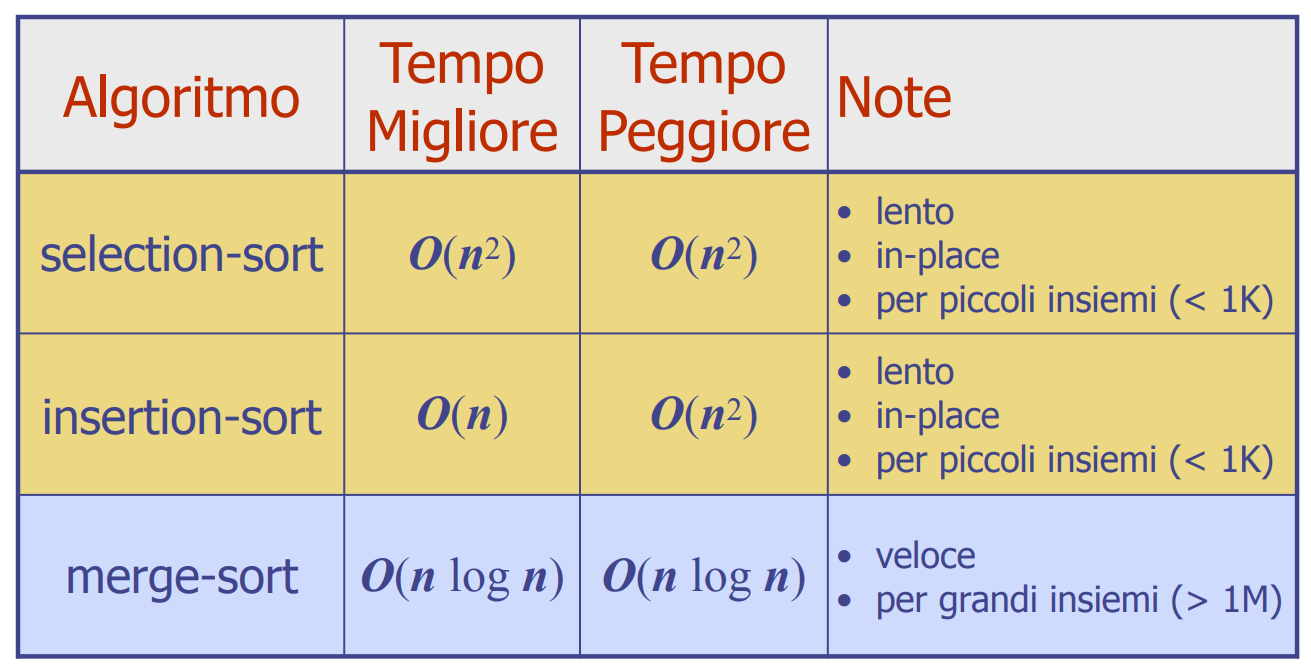
\includegraphics[width=0.8\textwidth]{costo_algo.png}
\end{center}

\pagebreak

\section{Alberi}
Un albero è un grafo connesso aciclico. I nodi di grado 1 sono detti foglie, i nodi di grado > 1 sono detti nodi interni.
Un albero \emph{radicato} ha 1 nodo \textbf{radice}.
I nodi interni hanno 1 o più filgi, che consideriamo ordinati e numerati da 0 a k.

Nel caso \(k = 2\) l'albero radicato è detto \textbf{binario}. In questo caso i filgi si chiamano sinistro (sx) e destro (dx).

\pagebreak

\section{Tempo di esecuzione}
\begin{align*}
    T(n) = n   &  & N_l = kT
    T(n) = n^2 &  & N_q = \sqrt[2]{kT}
    T(n) = n^3 &  & N_c = \sqrt[3]{kT}
\end{align*}

\section{Scoping}
Il campo di azione di un identificatore, detto scope, è la porzione di programma in cui l'identificatore può essere utilizzato. \emph{Block-Scope} significa che gli identificatori possono essere utilizzati nel blocco di programma in cui sono definiti, e in eventuali \emph{sotto-blocchi}.
Gli identificatori dichiarati sono \textbf{identificatori legati} e le dichiarazioni sono \textbf{occorrenze di legame}.
\begin{dfn}{Scoping statico}
    Tecnica di scoping basata sull'albero di sintassi che non richiede l'esecuzione del codice per controllarne la validità.
\end{dfn}
\begin{dfn}{Scoping dinamico}
    Tecnica di scoping che analizza il codice a tempo di esecuzione stabilendo i legami attraverso l'ambiente.
\end{dfn}
Possiamo quindi partizionare gli identificatori in \textbf{liberi} e \textbf{legati} in base alle regole di scoping.

\pagebreak
\section{Funzioni}
Le funzioni ci permettono di applicare il principio di astrazione, ovvero di ridurre la duplicazione di informazione nei programmi, facilitndo la comprensione e menutenzione del codice. Le funzioni consentono
\begin{itemize}
    \item modularità
    \item chiarezza e leggibilità
    \item fattorizzazione del codice
    \item separazione tra utilizzo e implementazione
\end{itemize}
Nell'utilzzo delle funzioni, distinguiamo due fasi diverse
\begin{itemize}
    \item \textbf{definizione di funzione}: definizione del codice che realizza l'operazione astratta
    \item \textbf{chiamata di funzione}: utilizzo della funzione attraverso un espressione
\end{itemize}

\subsection{Definizione di funzione}

\subsection{Chiamata di funzione}
La chiamata di funzione è un espressione che viene valutatà così
\begin{enumerate}
    \item viene sospesa l'esecuzione del chiamante e vengono assegnati i parametri attuali a quelli formali
    \item esecuzione di F
    \item istruzione return che termina l'esecuzione di F
    \item il controllo ritorna al chiamante, e la chiamata ad F assume il valore \quoted{calcolato} dal return
\end{enumerate}




\end{document}